\documentclass[12pt,a4paper]{article}
\usepackage[utf8]{inputenc}

\usepackage{mathtools}
\usepackage{amsmath}
\usepackage{amssymb}
\usepackage{amsthm}
\usepackage{amssymb}
\usepackage{mathdots}
\usepackage[pdftex]{graphicx}
\usepackage{fancyhdr}
\usepackage[margin=1in]{geometry}
\usepackage{multicol}
\usepackage{bm}
\usepackage{listings}
\usepackage{xcolor}
\usepackage{pdfpages}
\usepackage{algpseudocode}
\usepackage{tikz}
\usepackage{enumitem}
\usepackage[T1]{fontenc}
\usepackage{enumitem}
\usepackage{inconsolata}
\usepackage{framed}
\usepackage{wasysym}
\usepackage[thinlines]{easytable}
\usepackage{hyperref}
\usepackage{minted}
\usemintedstyle{perldoc}
\hypersetup{
    colorlinks=true,
    linkcolor=blue,
    filecolor=magenta,      
    urlcolor=blue,
}
\definecolor{codegreen}{rgb}{0,0.6,0}
\definecolor{codegray}{rgb}{0.5,0.5,0.5}
\definecolor{codepurple}{rgb}{0.58,0,0.82}
\definecolor{backcolour}{rgb}{0.95,0.95,0.92}
\lstdefinestyle{mystyle}{
    backgroundcolor=\color{backcolour},   
    commentstyle=\color{codegreen},
    keywordstyle=\color{magenta},
    numberstyle=\tiny\color{codegray},
    stringstyle=\color{codepurple},
    basicstyle=\ttfamily,
    breakatwhitespace=false,         
    breaklines=true,                 
    captionpos=b,                    
    keepspaces=true,                 
    numbers=left,                    
    numbersep=5pt,                  
    showspaces=false,                
    showstringspaces=false,
    showtabs=false,                  
    tabsize=4
}
\lstset{style=mystyle}
\newcommand\numberthis{\addtocounter{equation}{1}\tag{\theequation}}
\newcommand{\rightqed}{
\begin{flushright}
$\blacksquare$
\end{flushright}
}
\newcommand{\solution}{\noindent\textbf{Solution:}\\}
\usepackage{graphics}
\graphicspath{ {./images/} }

\title{CSCI 6550 Artificial Intelligence Homework 1}
\author{Kushajveer Singh}
\date{}

\begin{document}
\maketitle

% Start problem 1
\subsection*{Part I}
\textit{
    Suppose a given problem has an infinite state space (and contains no cycles). Assume negative step-costs are allowed, all step-costs are integer values and they are all the same. Branching is finite. All goal states are reachable from the start state.
}

\solution
\textbf{(a) Breadth-First Search}

BFS is guaranteed to find a solution but the solution may not be optimal. BFS is complete because it will look at all states at depth $d$ and then look at all states at depth $d+1$ and so on. So BFS is guaranteed to find the goal state as in the worst case it would explore all the states. The solution may not be optimal, because BFS is not using the path cost to make its decision. An easy counterexample is the case when the shortest path (as BFS returns shortest path) is not the minimum cost path.

\noindent\textbf{(b) Uniform Cost Search}

UCS is guaranteed to find a solution but the solution may not be optimal. UCS is guaranteed to terminate because in the worst case it would explore all the states. But the solution may not be optimal. UCS would terminate when it reaches the goal state. But because negative costs are allowed there may be cases where another path with more negative costs at the end can make the overall path cost less than the solution found by UCS. Thus, UCS would have to explore all the states before termination in order to find an optimal solution.

\noindent\textbf{(c) $A^*$}

$A^*$ is guaranteed to find a solution but the solution may not be optimal. In the worst case $A^*$ can visit all the states if needed. $A^*$ uses a heuristic function to estimate an approximate cost from a give state to goal state. For $A^*$ to be optimal the heuristic has to be consistent which requires the following condition to be met $h(n') \leq h(n) + c(n,n')$. Suppose n is a good state but n' is a bad state which means h(n) would be low and h(n') would be high. In order for the above equation to hold true the cost has to be positive in this case but there may be cases when moving from state n to n' has negative step cost, which would make the heuristic inconsistent. As we cannot find a consistent heuristic, $A^*$ is not guaranteed to find an optimal solution.

\noindent\textbf{(d) Iterative Deepening}

Iterative deepening is guaranteed to find a solution but the solution may not be optimal. Iterative deepening is essentially a combination of BFS and DFS. As it is an uninformed search algorithms i.e. it does not make use of step cost to guide the search, the path found by iterative deepening is not always guaranteed to be optimal. Suppose iterative deepening found a solution at depth $d$ but there is a possibility that the optimal solution occurs at depth $k$ (k > d) with path cost smaller than the solution found at depth $d$.

\newpage
\subsection*{Problem 1}
\textit{
    Answer True/False
}

\solution
    
(a) False, because there might be a case when the minimum cost path is longer than the shortest path, in which case $A^*$ would explore states that lead to minimum cost path. As DFS does not make use of path costs in its decision on which states to explore, it might be the case that the DFS explores the shortest path based on random luck (e.g. shortest path is the left most leaf of a graph search problem).

(b) True, an admissible heuristic is one that never overestimates the true minimum. As zero is the minimum value, thus $h(n) = 0$ can never overestimate the true minimum from n's state to a goal state.

(c) True, because breadth first search does not make use of step costs to guide its search. BFS explores all the states at a given depth before moving to the next depth and thus it can explore all the states if needed.

(d) False, if rook moves 4 squares in a single step, the manhattan distance would be 4 but the rook only took 1 step to move. So the heuristic is overestimating the true minimum value and thus is not admissible.

(e) False, because the heuristic is overestimating the true minimum. To move a chess piece from (1,1) to (2,2) we require minimum 1 step (the diagonal step) but the manhattan distance would be 2, which is greater than the true minimum and thus the heuristic is not admissible.

\newpage
\subsection*{Problem 2}
\textit{
    Consider a state space where the start state is number 1 and each state k has two successors: numbers 2k and 2k + 1.
}

\solution
\noindent\textbf{(a)}
\begin{figure}[H]
    \centering
    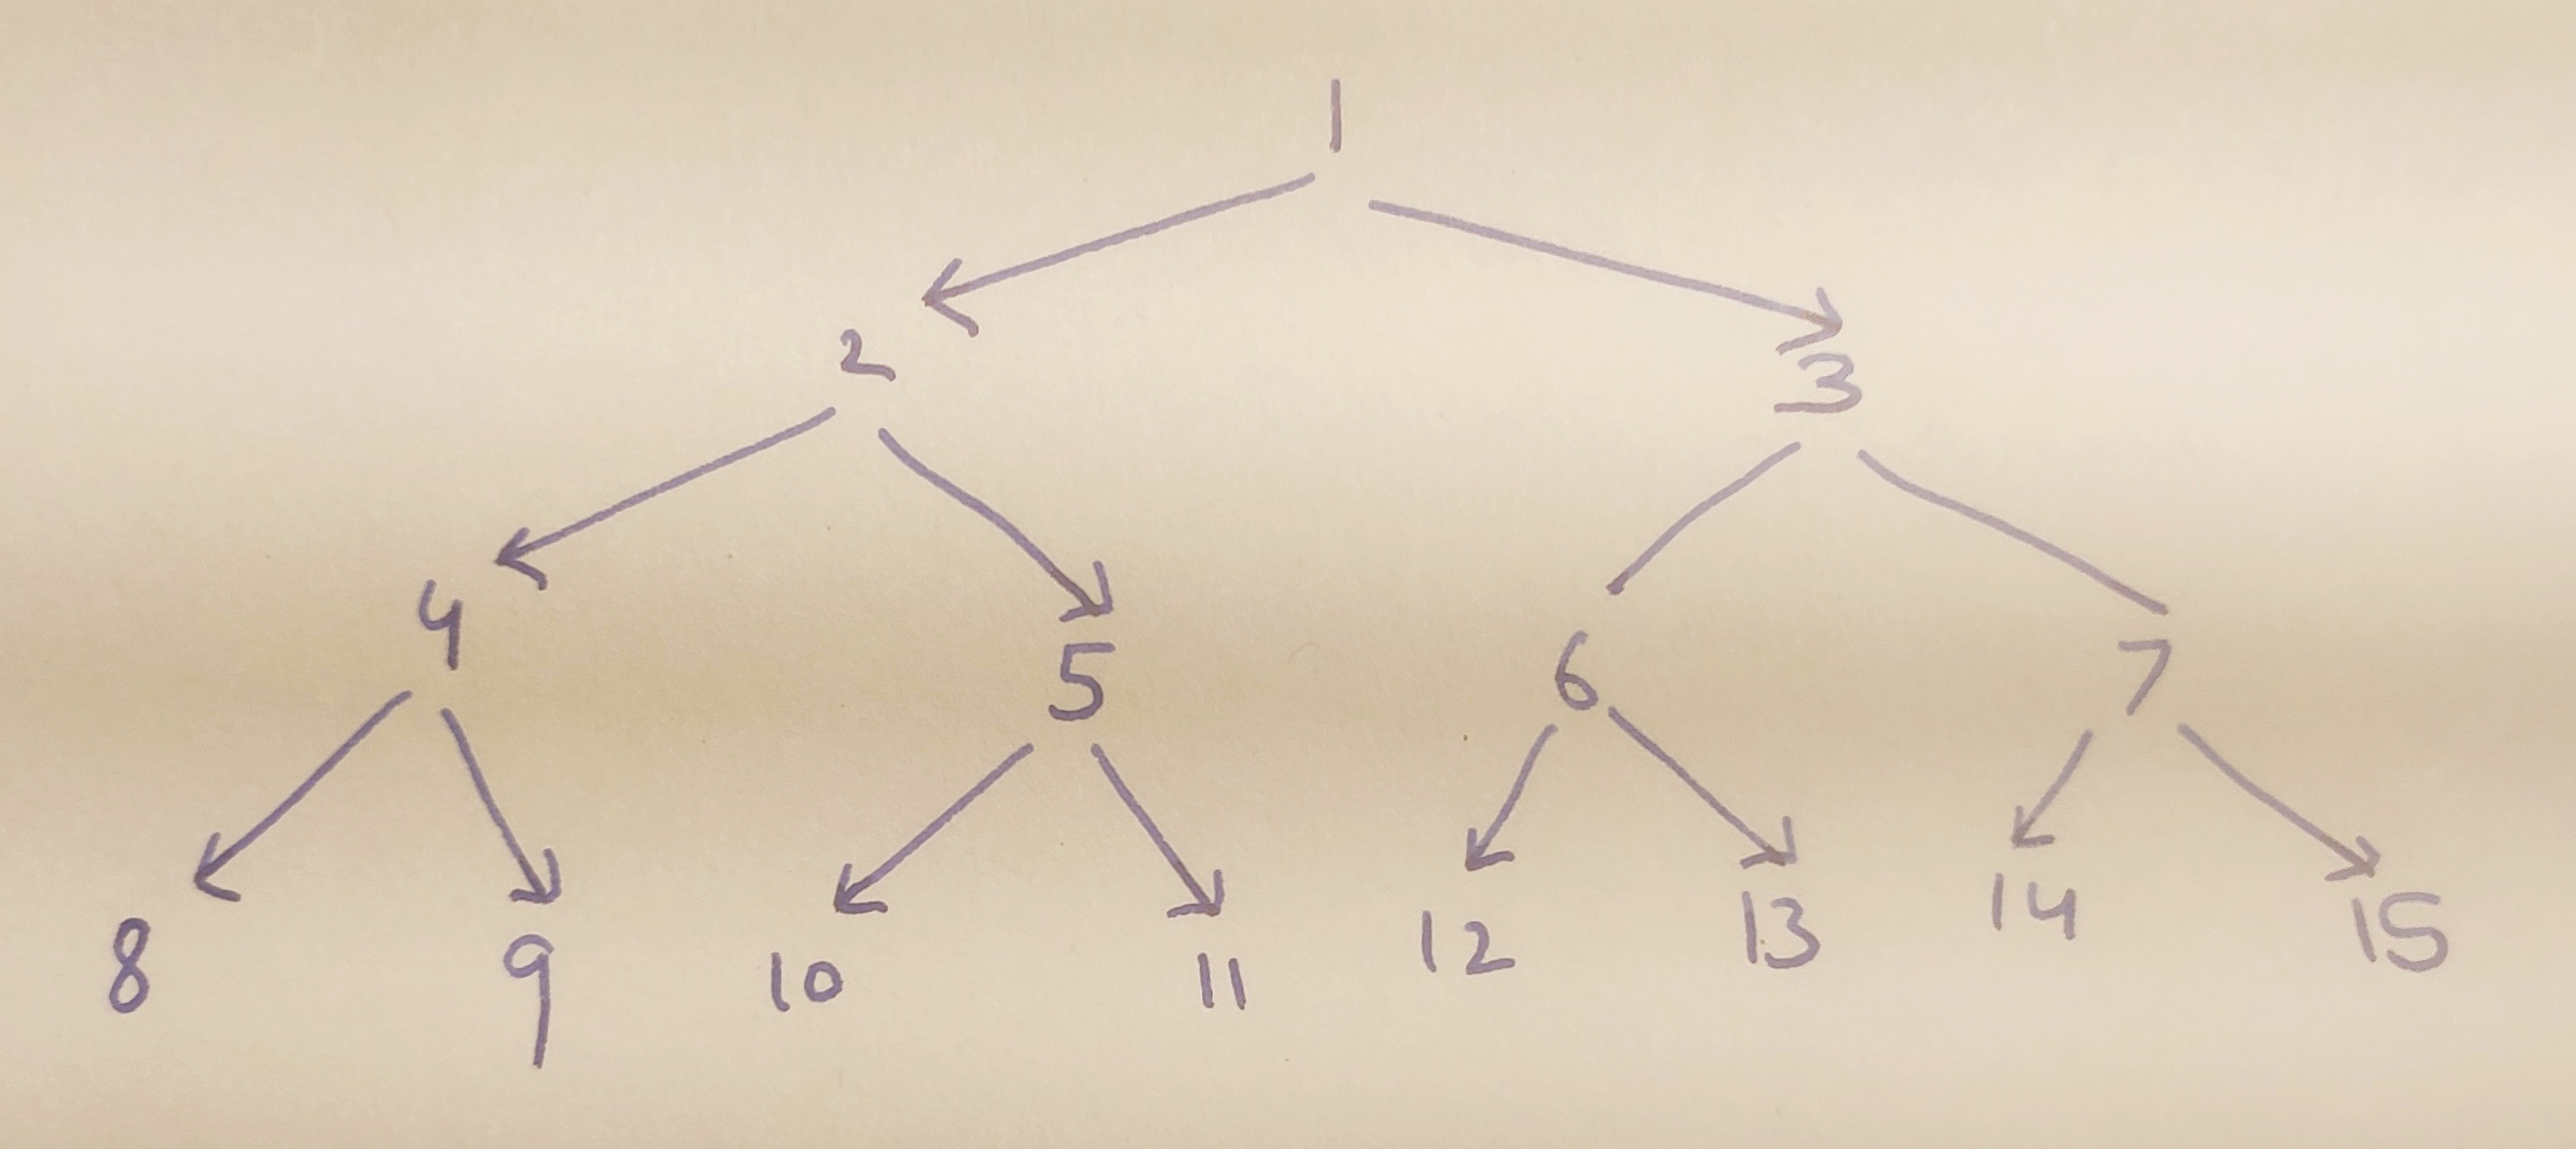
\includegraphics[width=12cm]{prob_2_a.jpg}
    \caption{Solution to Problem 2(a)}
\end{figure}

\noindent\textbf{(b)}
Breadth first search = [1, 2, 3, 4, 5, 6, 7, 8, 9, 10, 11]

Depth limited search = [1, 2, 4, 8, 9, 5, 10, 11] 

Iterative deepening search  = [1, 1, 2, 3, 1, 2, 4, 5, 3, 6, 7, 1, 2, 4, 8, 9, 5, 10, 11]

\noindent\textbf{(c)} Bidirectional search would work really well on this problem. The branching factor is 2 in both directions except for the leaf  and root states in which case it is 1 (in the reverse direction).

Performing BFS from both directions we observe the following order in which states are explored [(1,11), (2, 5), (3, 2)]. (1,11) means the forward step explored state 1 and backward step explored state 11. As we can see bidirectional search found a solution in 3 steps (3 forward, 3 backward).

\subsection*{Part II (A)}
\textit{
    Implement DFS and BFS.
}

\solution
Both BFS and DFS return a single path i.e. $[0, 2, 4, 8, 10, 11, 14, 16, 17]$. The code for BFS is in $bfs.py$ and code for dfs is in $dfs.py$ written in Python 3.8.

\end{document}
